\section{Problem, Related Work, and Methodology}
\label{sec:ipsn-problem}

In this section, we describe our model of the shared spectrum systems,
formulate the \mtl problem, and discuss related work.  We also
describe the building block of our approach, viz., a hypothesis-drived
Bayesian localization approach (\map).

\para{Shared Spectrum System.} In a shared spectrum paradigm, the
spectrum is shared among licensed users (primary users, PUs) and
unlicensed users (secondary users, SUs) in such a way that the
transmission from secondaries does not interfere with that of the
primaries (or secondaries from a higher-tier, in case of a multi-tier
shared spectrum system~\cite{scte-isbe16-cbrs}). In some shared spectrum systems,
the location and transmit power of the primary users may be
unavailable, as is the case with military or navy radars in the CBRS
band~\cite{scte-isbe16-cbrs}.
%%%%%
Such sharing of spectrum is generally orchestrated by a centralized
entity called {\em spectrum manager}, such as a spectrum
database in TV white
space~\cite{sas-paper} or a central spectrum access system in
the CBRS 3.5GHz shared band~\cite{milind2015dyspan}. The spectrum
manager allocates spectrum to requesting secondaries (i.e., permission
to transmit up to a certain transmit power at their location) based on
their location, spectrum demand, configurations of the primaries, other
active secondaries, prevailing channel conditions, etc.

\para{Authorized and Unauthorized Users.}
Secondary users that have been explicitly given permission to transmit
at their location are termed as {\em authorized users}; the primaries
users are also considered as authorized users. Note that the set of
authorized users evolve over time, as more and more SUs are allocated
spectrum and as some SUs stop using the spectrum after a while. We can
assume that each SU is allocated spectrum for a certain duration of
time, after which it stops using the spectrum. 
%%%%%%%%%%%%
Other users that transmit without explicit permission (for that given
time) are referred to as {\em unauthorized users} or {\em intruders}.

\para{Problem Setting and Formal Definition.}  Consider a geographic
area with a shared spectrum. Without loss of generality, we assume a
single channel throughout this paper (multiple channels are handled
similarly). For localization of unauthorized users, we assume
available crowdsourced sensors that can observe received signal in the
channel of interest, and compute (totel) received signal strength
indicator (RSSI)\footnote{We do not use angle-of-arrival (AoA)
    measurements~\cite{aoa-multi} as they require additional and
    complex RF hardware.}. These sensors, being crowdsourced, may be at
  different locations at different times.  At any given instant, the
  shared spectrum area has some licensed primary users and some active
  secondary users; the PU configurations may not be known as can be
  the case for military users. The centralized spectrum manager is
  aware of the set of active SUs at any time, as each SU request is
  granted for a certain period of time.
%%%%
In addition to the authorized users, there may be a set of intruders
present in the area with each intruder in a certain ``configuration''
(see \S\ref{sec:map}).

The \mtl problem is to determine the set of intruders with their
configurations at each instant of time, based on the set of sensor
observations at that instant. See Figure \ref{fig:ipsn-illustration}. 
The basic \mtl problem assumes no other
transmissions (of authorized users) in the background.
%%%%%
The more general \mtl problem, where there may be an evolving set of
authorized users in the background, is referred to as the \mtlss
problem.  We address the \mtl problem in~\S\ref{sec:map-time}, and
then address the more general \mtlss problem in~\S\ref{sec:mtlss}.

%% Let $\theta_i = (l_i, p_i)$ denotes the configuration of location and
%% power of one transmitter, and $\boldsymbol{\theta_M} = \{\theta_1,
%% \theta_2, \cdots, \theta_M \}$ denotes the configurations of all
%% intruders. 
%% The problem is to predict $\boldsymbol{\theta_M}$ based on the observed received power
%% reported by sensor $\vx = \{x_1, x_2, \cdots, \}$.

\subsection{Related Work}
\label{sec:ipsn-related}

Localization of an intruder in a field using sensor observations has
been widely studied, but most of the works have focused on
localization of a single intruder~\cite{infocom18-spectrum,dutta2016see}.
%%%%%
In general, to localize multiple intruders, the main challenge comes
from the need to ``separate'' powers at the sensors~\cite{mobicom-30},
i.e., to divide the total received power into power received from
individual intruders. Blind source separation is a very challenging
problem; only very limited settings allow for known
techniques~\cite{freq-sig,ben-zhao} using sophisticated receivers. In
our context of hypotheses-driven approach, the challenge of source
separation manifests in terms of a large number of hypotheses, a
challenge addressed in~\S\ref{sec:map-time}.
%%%
We note that (indoor) localization of a
  device~\cite{infocom00-radar} based on signals received from multiple reference points (e.g, WiFi access
  points) is a quite different problem
  (see~\cite{zafari-19} for a recent survey), as the signals from
  reference points remain separate, and localization or tracking of multiple
  devices can be done independently.
  Recent works on multi-target localization/tracking are different in the way that targets are passive~\cite{ipsn19-multipassive, ipsn19-chorus, ipsn19-snaploc}, instead of active transmitters in this work.

In absence of blind separation methods, to the best of our knowledge,
only a few works have addressed multiple intruder(s) localization, and
none of these consider it in the presence of a dynamically changing
set of authorized transmitters. In particular,
(i)~\cite{mobicom17-splot} decomposes the multi-transmitter
localization problem to multiple single-transmitter localization
problems based on the sensors with highest of readings in a
neighbohood, (ii)~\cite{clustering} works by clustering the sensors
with readings above a certain threshold and then localizing intruders
at the centers of these clusters, (iii)~\cite{Quasi-EM} uses an
EM-based approach.
%%%
The techniques of~\cite{mobicom17-splot,Quasi-EM} assume a propagation
model, while that of~\cite{clustering,Quasi-EM} require a priori
knowledge of the number of intruders present.  We have compared our
approach with~\cite{mobicom17-splot,clustering} in \S\ref{sec:eval},
while~\cite{Quasi-EM} has high computational cost and has also been
shown to be inferior in performance
to~\cite{mobicom17-splot,clustering} even for a small number of
intruders. Other related works include
  (i)~\cite{multi-tx-dyspan-19} that addresses the challenge of
  handling time-skewed sensors observations in the MTL problem, and
  (ii)~\cite{info-20} that addresses the sensor selection optimization
  problem for our proposed hypotheses-based localization approach.
  
%%%%%
%\blue{Other related works include:~\cite{mobicom-22} where sensors are
%  on mobile and controlled robots,~\cite{mobi-25} focusses on spectrum
%  allocation via spectrum hole detection in presence of background 
%  transmitters.} \red{HG: Remove this sentence?}

%% Online selection of sensors: ipsn-04, .... latency vs. energy .. since,
%% latency is equally critical, ... we dont want to run it for every intruder ... 
%% Similarly,
%% \cite{krause2008near} shows that minimizing uncertainty in a gaussian
%% process is submodular, and thus greedy selection provides a bounded
%% solution to the optimal.

%% Multiple studies have studied sensor selection to maximize the
%% accuracy of detection of some event \cite{rowaihy2007survey}.

%% For
%% example, \cite{joshi2009sensor} provides a heuristic for sensor
%% selection by forming a convex optimization problem.  However, it uses
%% a different metric to measure the accuracy of detection.
%% %%%%
%% Other studies, such as
%% \cite{shamaiah2010greedy} and \cite{bian2006utility} have proposed
%% leveraging submodularity to select sensors.  

%% There are also studies in the active learning literature that focus on
%% online selection.  For example, \cite{yuxin-when} limits the mutual
%% information while selecting the minimum possible number of sensors.
%% \cite{krause2012near} shows that mutual information in sensor
%% selection is submodular in the absence of noise and propose a
%% probabilistic greedy algorithm by leveraging it.
%% \cite{golovin2011adaptive} proposes the concept of adaptive
%% submodularity that generalizes the greedy approximation to online
%% selection. Our online selection algorithm builds upon these studies to
%% limit the number of sensors while maximizing the mutual information.
%% However, in the presence of noise, mutual information is not adaptive
%% submodular in nature.  Thus, our work modifies the algorithm discussed
%% in \cite{yuxin-when} to make it suitable for our use case.


\subsection{\map: Bayesian Approach for Localization}
\label{sec:map}

We localize intruders based on observations from a set of
sensors. Each sensor communicates its observation to a centralized
entity, the spectrum manager, which runs an appropriate
localization algorithm to localize the intruders.
%%%%
In particular, we use a hypotheses-driven Bayesian approach, as
described below, where intruders are localized by determining the
most-likely prevailing hypothesis; this is done based on joint
probability distributions of the sensors' observations (constructed
during a priori training). Below, we formalize the above concepts, and
the basic localization approach.

\para{Observation; Observation Vector.} Throughout this
paper, we use the term {\em observation} at an individual sensor to
mean the received power over a time window of certain duration, in the
frequency channel of interest (we assume only one channel). In
particular, received power is computed from the FFT of the I/Q samples
in the time window~\cite{arani2018}. We use the term {\em observation
  vector} \vx to denote a vector of observations from a given set of
distributed sensors, with each vector dimension corresponding to a
unique sensor.
%%%%%%%%
%% We assume a Gaussian distribution $N (\mu, \sigma^2)$ for each
%% observation, where mean implies the average power the receiver
%% receive, and standard deviation will represent the noise, shadowing,
%% and multi-path fading.

\begin{wrapfigure}{r}{2in}
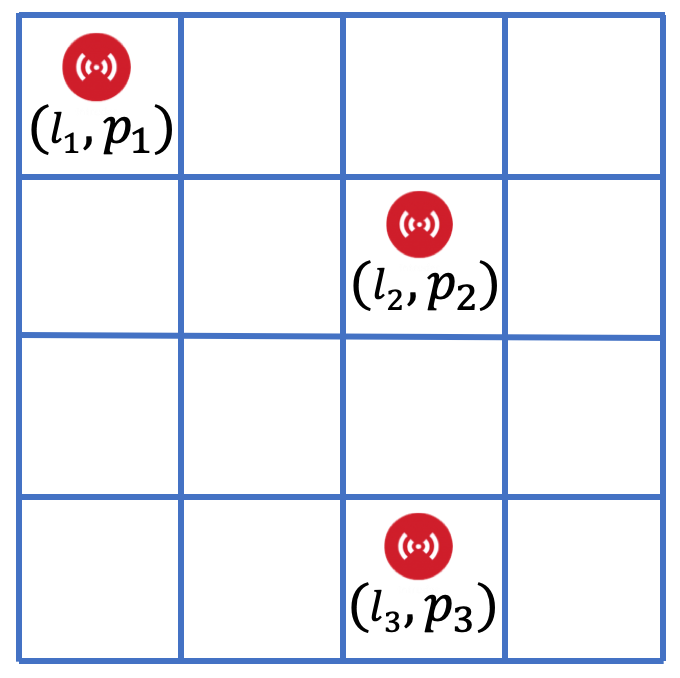
\includegraphics[width=2in]{chapters/ipsn/figures/hypothesis.png}
\caption{Illustration of a hypothesis formed of three transmitters.}
\label{fig:hypothesis-grid}
\end{wrapfigure}
\para{Hypotheses.} Let \hz, \ho, $\ldots,$ \hM be the set of all
hypotheses, where each hypothesis \hj represents a ``configuration''
of potential intruders. In this chapter, we largely assume an
  intruder's configuration to be comprised of just its location and
  transmit power, but the concept of configuration is quite general
  and could include any attributes (e.g., height, antenna direction,
  etc.) that affects how its transmitted signal is received at other
  locations. Moreover, for simplicity, we assume that each intruder
  transmits at a fixed power (which may be different for different
  intruders). Thus, in our context, a configuration is simply the set
of (location, transmit power) pairs of the potential intruders. We
assume a bounded number of intruders. We use \hz to represent the
hypothesis with no intruders. See Figure~\ref{fig:hypothesis-grid}.

%%%%%%%
If there is only one intruder, then each hypothesis represents the
location and transmit power combination of the intruder, and
determining the hypothesis is equivalent to localizing the intruder
and estimating its power. If we allow multiple intruders at a time,
the number of possible hypotheses can be exponential in the number of
intruders; we will address this challenge in
\S\ref{sec:map-time}.

\softpara{Inputs.} For a given set of sensors deployed over an area, we
assume the following available inputs, obtained via a priori training,
data gathering and/or analysis:
\begin{itemize}
\item
Prior probabilities of the hypotheses, i.e. $P(H_i)$, for each
hypothesis $H_i$. Prior probabilities come from known knowledge about
area, intruder's behavior, etc., and can be assumed to be uniform in
absence of better knowledge.

\item
Joint probability distribution (JPD) of sensors' observations for each
hypothesis. More formally, for each hypothesis $H_j$, we assume
$P(\vx|H_j)$ to be known for each observation $\vx$ for the set of
deployed sensors.  The JPDs can be obtained from prior training, a
combination of training and interpolation (\S\ref{sec:inter}), or
even by assuming a propagation model to remove the training
cost completely.
\end{itemize}

\para{Maximum a Posteriori (\mll) Localization Algorithm.}  We use
Bayes rule to compute the likelihood probability of each hypothesis,
from a given observation vector $\vx$:
\begin{equation}
  P(H_i | \vx) = \frac{P(\vx| H_i)P(H_i)}{\sum_{j=0}^m P(\vx|H_j)P(H_j)}
  \label{eqn:bayes}
\end{equation}
We select the hypothesis that has the highest probability, for given
observations of a set of sensors. That is, the \mll Algorithm returns
the hypotheses based on the following equation:
\begin{equation}
  \arg \max_{i=0}^m P(H_i | \vx)
  \label{eqn:map}
\end{equation}
The above \mll algorithm to determine the prevailing hypothesis is
known to be {\em optimal}~\cite{map-optimal}, i.e., it yields minimum
probability of (misclassification) error. The above hypothesis-based
approach to localization works for arbitrary signal propagation
characteristics, and in particular, obviates the need to assume a
propagation model. However, the above \mll algorithm does incur a {\em
  one-time} training cost to construct the JPDs.



